% Options for packages loaded elsewhere
\PassOptionsToPackage{unicode}{hyperref}
\PassOptionsToPackage{hyphens}{url}
%
\documentclass[
]{book}
\usepackage{lmodern}
\usepackage{amssymb,amsmath}
\usepackage{ifxetex,ifluatex}
\ifnum 0\ifxetex 1\fi\ifluatex 1\fi=0 % if pdftex
  \usepackage[T1]{fontenc}
  \usepackage[utf8]{inputenc}
  \usepackage{textcomp} % provide euro and other symbols
\else % if luatex or xetex
  \usepackage{unicode-math}
  \defaultfontfeatures{Scale=MatchLowercase}
  \defaultfontfeatures[\rmfamily]{Ligatures=TeX,Scale=1}
\fi
% Use upquote if available, for straight quotes in verbatim environments
\IfFileExists{upquote.sty}{\usepackage{upquote}}{}
\IfFileExists{microtype.sty}{% use microtype if available
  \usepackage[]{microtype}
  \UseMicrotypeSet[protrusion]{basicmath} % disable protrusion for tt fonts
}{}
\makeatletter
\@ifundefined{KOMAClassName}{% if non-KOMA class
  \IfFileExists{parskip.sty}{%
    \usepackage{parskip}
  }{% else
    \setlength{\parindent}{0pt}
    \setlength{\parskip}{6pt plus 2pt minus 1pt}}
}{% if KOMA class
  \KOMAoptions{parskip=half}}
\makeatother
\usepackage{xcolor}
\IfFileExists{xurl.sty}{\usepackage{xurl}}{} % add URL line breaks if available
\IfFileExists{bookmark.sty}{\usepackage{bookmark}}{\usepackage{hyperref}}
\hypersetup{
  pdftitle={RCE Quick-Start Guide},
  hidelinks,
  pdfcreator={LaTeX via pandoc}}
\urlstyle{same} % disable monospaced font for URLs
\usepackage[margin=1.5in]{geometry}
\usepackage{color}
\usepackage{fancyvrb}
\newcommand{\VerbBar}{|}
\newcommand{\VERB}{\Verb[commandchars=\\\{\}]}
\DefineVerbatimEnvironment{Highlighting}{Verbatim}{commandchars=\\\{\}}
% Add ',fontsize=\small' for more characters per line
\usepackage{framed}
\definecolor{shadecolor}{RGB}{248,248,248}
\newenvironment{Shaded}{\begin{snugshade}}{\end{snugshade}}
\newcommand{\AlertTok}[1]{\textcolor[rgb]{0.94,0.16,0.16}{#1}}
\newcommand{\AnnotationTok}[1]{\textcolor[rgb]{0.56,0.35,0.01}{\textbf{\textit{#1}}}}
\newcommand{\AttributeTok}[1]{\textcolor[rgb]{0.77,0.63,0.00}{#1}}
\newcommand{\BaseNTok}[1]{\textcolor[rgb]{0.00,0.00,0.81}{#1}}
\newcommand{\BuiltInTok}[1]{#1}
\newcommand{\CharTok}[1]{\textcolor[rgb]{0.31,0.60,0.02}{#1}}
\newcommand{\CommentTok}[1]{\textcolor[rgb]{0.56,0.35,0.01}{\textit{#1}}}
\newcommand{\CommentVarTok}[1]{\textcolor[rgb]{0.56,0.35,0.01}{\textbf{\textit{#1}}}}
\newcommand{\ConstantTok}[1]{\textcolor[rgb]{0.00,0.00,0.00}{#1}}
\newcommand{\ControlFlowTok}[1]{\textcolor[rgb]{0.13,0.29,0.53}{\textbf{#1}}}
\newcommand{\DataTypeTok}[1]{\textcolor[rgb]{0.13,0.29,0.53}{#1}}
\newcommand{\DecValTok}[1]{\textcolor[rgb]{0.00,0.00,0.81}{#1}}
\newcommand{\DocumentationTok}[1]{\textcolor[rgb]{0.56,0.35,0.01}{\textbf{\textit{#1}}}}
\newcommand{\ErrorTok}[1]{\textcolor[rgb]{0.64,0.00,0.00}{\textbf{#1}}}
\newcommand{\ExtensionTok}[1]{#1}
\newcommand{\FloatTok}[1]{\textcolor[rgb]{0.00,0.00,0.81}{#1}}
\newcommand{\FunctionTok}[1]{\textcolor[rgb]{0.00,0.00,0.00}{#1}}
\newcommand{\ImportTok}[1]{#1}
\newcommand{\InformationTok}[1]{\textcolor[rgb]{0.56,0.35,0.01}{\textbf{\textit{#1}}}}
\newcommand{\KeywordTok}[1]{\textcolor[rgb]{0.13,0.29,0.53}{\textbf{#1}}}
\newcommand{\NormalTok}[1]{#1}
\newcommand{\OperatorTok}[1]{\textcolor[rgb]{0.81,0.36,0.00}{\textbf{#1}}}
\newcommand{\OtherTok}[1]{\textcolor[rgb]{0.56,0.35,0.01}{#1}}
\newcommand{\PreprocessorTok}[1]{\textcolor[rgb]{0.56,0.35,0.01}{\textit{#1}}}
\newcommand{\RegionMarkerTok}[1]{#1}
\newcommand{\SpecialCharTok}[1]{\textcolor[rgb]{0.00,0.00,0.00}{#1}}
\newcommand{\SpecialStringTok}[1]{\textcolor[rgb]{0.31,0.60,0.02}{#1}}
\newcommand{\StringTok}[1]{\textcolor[rgb]{0.31,0.60,0.02}{#1}}
\newcommand{\VariableTok}[1]{\textcolor[rgb]{0.00,0.00,0.00}{#1}}
\newcommand{\VerbatimStringTok}[1]{\textcolor[rgb]{0.31,0.60,0.02}{#1}}
\newcommand{\WarningTok}[1]{\textcolor[rgb]{0.56,0.35,0.01}{\textbf{\textit{#1}}}}
\usepackage{longtable,booktabs}
% Correct order of tables after \paragraph or \subparagraph
\usepackage{etoolbox}
\makeatletter
\patchcmd\longtable{\par}{\if@noskipsec\mbox{}\fi\par}{}{}
\makeatother
% Allow footnotes in longtable head/foot
\IfFileExists{footnotehyper.sty}{\usepackage{footnotehyper}}{\usepackage{footnote}}
\makesavenoteenv{longtable}
\usepackage{graphicx}
\makeatletter
\def\maxwidth{\ifdim\Gin@nat@width>\linewidth\linewidth\else\Gin@nat@width\fi}
\def\maxheight{\ifdim\Gin@nat@height>\textheight\textheight\else\Gin@nat@height\fi}
\makeatother
% Scale images if necessary, so that they will not overflow the page
% margins by default, and it is still possible to overwrite the defaults
% using explicit options in \includegraphics[width, height, ...]{}
\setkeys{Gin}{width=\maxwidth,height=\maxheight,keepaspectratio}
% Set default figure placement to htbp
\makeatletter
\def\fps@figure{htbp}
\makeatother
\setlength{\emergencystretch}{3em} % prevent overfull lines
\providecommand{\tightlist}{%
  \setlength{\itemsep}{0pt}\setlength{\parskip}{0pt}}
\setcounter{secnumdepth}{5}
\usepackage{booktabs}

\usepackage{epsfig}
\usepackage{epstopdf}
\usepackage{rotate}
\usepackage{graphicx}
\usepackage{hyperref}
\usepackage{alphalph}
\usepackage{caption}
\usepackage[hang,flushmargin]{footmisc}
\usepackage{framed}
\usepackage{xcolor}
\usepackage{verbatim} 

\usepackage{bm}
\setcounter{MaxMatrixCols}{20}
\newcommand{\Var}{\mathrm{Var}}
\newcommand{\SD}{\mathrm{SD}}
\newcommand{\Cov}{\mathrm{Cov}}
\newcommand{\fx}{f({\bf x})}
\newcommand\R{{\textsf R~}}
\newcommand\Rst{\textsf{RStudio}}

% spacing between environments
\usepackage{amsthm}
\makeatletter
\def\thm@space@setup{%
  \thm@preskip=15pt plus 2pt minus 4pt
  \thm@postskip=\thm@preskip
}
\makeatother


% Title format
\usepackage{titling}
\pretitle{\Huge\sffamily}
\posttitle{\par\vskip 0.5em}
\predate{\LARGE\sffamily}
\postdate{\par}

\urlstyle{tt}
\usepackage[]{natbib}
\bibliographystyle{apalike}

\title{RCE Quick-Start Guide}
\author{}
\date{\vspace{-2.5em}January 2021}

\begin{document}
\maketitle

{
\setcounter{tocdepth}{1}
\tableofcontents
}
\hypertarget{what-is-the-rce}{%
\chapter*{What is the RCE?}\label{what-is-the-rce}}
\addcontentsline{toc}{chapter}{What is the RCE?}

The Research Computing Environment (RCE) is a powerful computer
cluster that you can use for computations that are too large to be
conveniently done on a personal computer. The RCE is available to
researchers at Harvard and MIT.

To obtain an RCE account send an email to
\href{mailto:help@iq.harvard.edu}{\nolinkurl{help@iq.harvard.edu}}. You will
receive a response asking you several questions about your requirements
(e.g., if you need backups, how much data storage space you need). For
details on the services provided and limitations and restrictions of the
service refer to
\url{http://projects.iq.harvard.edu/user-services/research-computing-environment-sla}.

You can use the RCE in one of two primary ways:

\begin{description}
\tightlist
\item[\textbf{Interactive jobs}]
Run your computation as you would on your PC, but on a much more
powerful machine with up to 24 CPU cores and up to 500Gb of memory.
\item[\textbf{Batch jobs}]
Run your computation in the background using up to several hundred
computers at once.
\end{description}

Interactive jobs are good for memory intensive computations that may be
unfeasible on your personal computer due to hardware limitations. Batch
jobs are good for computations that can be run in parallel and/or
computations that you expect to run for long periods of time.

\hypertarget{authors}{%
\section*{Authors}\label{authors}}
\addcontentsline{toc}{section}{Authors}

This tutorial was created by Ista Zahn and Steve Worthington at the Institute for Quantitative Social Science at Harvard University. Any comments or suggestions can be sent to: \href{mailto:help@iq.harvard.edu}{\nolinkurl{help@iq.harvard.edu}}.

\hypertarget{rce-setup}{%
\chapter{RCE Setup}\label{rce-setup}}

\hypertarget{access}{%
\section{Access}\label{access}}

You can access the RCE using the
\href{http://projects.iq.harvard.edu/rce/nx4_installation}{NoMachine} remote
desktop software, or via the command line using \texttt{ssh}. If you are a
command line wizard and only need to run batch jobs \texttt{ssh} is the way to
go; for most of us however \texttt{nomachine} is a much more useful way to
access the RCE. It allows you to interact with the applications on the
cluster much as you interact with applications on your local computer.

To get started, download the NoMachine client for your operating system:

\begin{itemize}
\tightlist
\item
  \href{http://downloads.hmdc.harvard.edu/nx/4/nomachine-client-windows-latest.zip}{Windows}
\item
  \href{http://downloads.hmdc.harvard.edu/nx/4/nomachine-client-osx-latest.dmg}{OSX}
\item
  \href{http://downloads.hmdc.harvard.edu/nx/4/nomachine-client-linux-latest.zip}{Linux}
\end{itemize}

After downloading, Windows users should right-click on the
\texttt{nomachine-client-windows-latest.zip} file and choose \texttt{Extract\ to\ here}.
Open the \texttt{NoMachine\ Client} folder and double-click on the .exe files to
start the installation (the Windows zipfile contains the NX client, plus optional
font packages. HMDC recommends installing all font packages, though
this is not required). Mac users should double-click on the
\texttt{nomachine-client-osx-latest.dmg} and double-click on the installer
package to begin the installation.

Once you have installed the NoMachine software you should launch the
NoMachine application and set up your login credentials.

Once the application launches:

\begin{itemize}
\tightlist
\item
  Click \texttt{Continue}.
\item
  Click \texttt{Click\ here\ to\ create\ a\ new\ connection}.
\item
  Keep clicking \texttt{Continue} until you get to the Hosts screen.
\item
  Fill in the Host field with \texttt{rce.hmdc.harvard.edu}.
\item
  Keep clicking \texttt{Continue} until you get to the Name screen.
\item
  Fill in the Name field with \texttt{RCE6} and click \texttt{Done}.
\end{itemize}

Once you have configured NoMachine you should test it out to make sure
you can connect to the RCE:

\begin{itemize}
\tightlist
\item
  Click on the \texttt{RCE6} entry and then click \texttt{Connect}.
\item
  Fill in the user name and password fields with your RCE user name and password.
\item
  On the following screen click on \texttt{New\ virtual\ desktop\ or\ custom\ session}.
\item
  Click on \texttt{Create\ a\ new\ virtual\ desktop} and click \texttt{Continue}.
\end{itemize}

After completing these steps you should see an instruction screen; click
\texttt{OK} and you should see your RCE desktop, which will look something like
this:


\includegraphics{images/rceDesktop.png}

If you have any difficulties installing NoMachine, detailed
documentation is available at \url{http://projects.iq.harvard.edu/rce/nx4};
if you do not find a solution there send and email to
\href{mailto:help@iq.harvard.edu}{\nolinkurl{help@iq.harvard.edu}} and someone will assist you.

\hypertarget{compute-nodes}{%
\section{Compute nodes}\label{compute-nodes}}

You can run applications on the RCE \emph{interactively} or using the \emph{batch}
system. If you simply want a more powerful version of your PC (e.g.,
more memory, more CPUs) then the interactive nodes are what you want. If
you want to split your task up into hundreds of pieces and run each
piece simultaneously, then you want the batch modes.

More specifically, the RCE provides three levels of service:

\begin{description}
\tightlist
\item[\textbf{Login nodes}]
Provides access to a desktop environment (similar to Remote Desktop)
from which you can launch applications. The login nodes should not
be used for computationally intensive jobs; the main function of the
login nodes is to provide access to the interactive and batch nodes.
You access the login nodes using the NoMachine client, as described
in \emph{Accessing the RCE}.
\item[\textbf{Interactive nodes}]
Interactive nodes allow you to run applications on very powerful
computers. You can launch applications on the interactive nodes from
the login node desktop using the
\texttt{Applications\ -\/-\textgreater{}\ RCE\ Powered\ Applications} menu. Applications
launched from this menu will run on more powerful machines with
large memory resources (up to 256GB) and up to 24 CPU cores.
\item[\textbf{Batch nodes}]
Where interactive nodes give you access to a single very powerful
computer, batch nodes provide a swarm of hundreds of small
computers. You can run your computation in parallel on each of them,
which can provide dramatically reduced compute time for many
applications. You access the batch nodes using the \emph{command line}
which you can access by starting a terminal application from the
\texttt{Applications\ -\/-\textgreater{}\ Accessories\ -\/-\textgreater{}\ terminal} menu.
\end{description}

\hypertarget{project-folders-shared-space}{%
\section{Project folders \& shared space}\label{project-folders-shared-space}}

When your RCE account was created a home folder was set up for you, with
\emph{Documents}, \emph{Downloads}, \emph{Desktop} and other common sub-directories.
However you can only store a maximum of 5Gb in your home folder. For
larger projects you should use a \emph{project folder}; one was probably set
up for you when your account was activated. There is a shortcut in your
home directory named \emph{shared space}, which will contain any project
folders you have access to. You should store large data sets and other
large or numerous files in these project folders.

Project space can be used privately, or shared with collaborators (hence
the name, `shared space'). For more details on project folders refer to
\url{http://projects.iq.harvard.edu/rce/book/projects-and-shared-space} and
\url{http://projects.iq.harvard.edu/rce/book/project-space-collaboration}.

\hypertarget{moving-your-data-on-and-off}{%
\section{Moving your data on and off}\label{moving-your-data-on-and-off}}

People often use the RCE for memory or CPU intensive data analysis
projects. If this is your intention as well, chances are that you have
one or more (potentially large) data files that you will need to copy to
the RCE. Remember that disk space in your home directory is limited, so
if you have a large amount of data make sure to \emph{transfer data directly
to your project space folder}.

The simplest approach is to use the NoMachine client to transfer data
from your local machine to the RCE (and from the RCE to your local
machine). Click on the red \texttt{!M} icon in the upper right-hand corner and
select the \texttt{Send\ a\ file\ from\ the\ client} menu, as shown below.

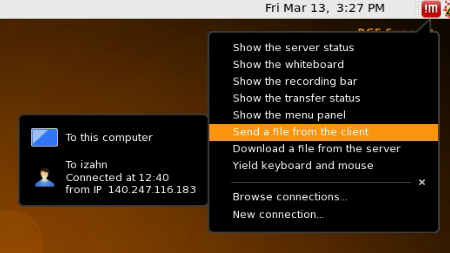
\includegraphics{images/NoMachineMenu.png}

If you prefer to transfer files using another file transfer client,
anything that uses ssh (e.g.,
\href{http://filezilla-project.org/}{FileZilla}) should work. Just point your
favorite client to \texttt{rce.hmdc.harvard.edu}.

\hypertarget{interactive-jobs}{%
\chapter{Interactive Jobs}\label{interactive-jobs}}

When you first log on to the RCE you are on a \emph{login node}. The login
nodes are not designed for intensive computation; the purpose of the
login nodes is to provide access to the \emph{interactive nodes} and the
\emph{batch nodes}. Interactive jobs are useful when a) you need a lot of
memory (e.g., because you need to load a large dataset into memory),
and/or b) you want to use multiple cores to speed up your computation.

\hypertarget{launching-applications}{%
\section{Launching applications}\label{launching-applications}}

Running applications on the interactive nodes is very easy; just log in
\emph{using NoMachine} and launch your application from the
\texttt{Application\ -\/-\textgreater{}\ RCE\ Powered} menu. A dialog will open asking you how
much memory you need and how many CPUs, and then your application will
open. That's all there is to it! Well, we should say that the RCE is a
shared resource, so please \emph{try not to request more memory or CPUs than
you need}. Also, applications running on the interactive nodes will
expire after five days; you can request an extension, but if you fail to
do so your job will be terminated 120 hours after it starts.

\hypertarget{available-applications}{%
\section{Available applications}\label{available-applications}}

Available RCE powered applications include:

\begin{itemize}
\tightlist
\item
  Gauss
\item
  Mathematica
\item
  Matlab/Octave
\item
  R/RStudio
\item
  SAS
\item
  Stata (MP and SE)
\item
  StatTransfer
\end{itemize}

Other applications (e.g., Python/IPython, perl, tesseract, various Unix
programs and utilities) can be run on the interactive nodes by launching
a terminal on an interactive node
(\texttt{Applications\ -\/-\textgreater{}\ RCE\ Powered\ -\/-\textgreater{}\ RCE\ Shell}) and launching your
program from the command line.

If you are using the interactive nodes primarily for the large memory
they provide you should have all the information you need to begin
taking advantage of the RCE. If you are also interested in using
multiple CPU cores to speed up your computations, read on! The following
sections contain examples illustrating techniques for utilizing multiple
cores on the RCE.

\hypertarget{using-multiple-cpus}{%
\section{Using multiple CPUs}\label{using-multiple-cpus}}

This section illustrates how to take advantage of multiple cores when
running interactive jobs on the RCE, with the goal of getting CPU
intensive tasks to run faster.

\hypertarget{r}{%
\subsection{R}\label{r}}

\begin{enumerate}
\def\labelenumi{\arabic{enumi}.}
\item
  Using multiple cores to speed up simulations

  Running computations in parallel on multiple cores is often an
  effective way to speed up computations. This can be especially
  useful when doing simulations, or when using resampling methods such
  as bootstrap or permutation tests. In this example parallel
  processing is used to simulate the sampling distribution of the mean
  for samples of various sizes.

  We start by setting up a helper function to repeatedly generate a
  sample of a given size and calculate the sample mean.

\begin{Shaded}
\begin{Highlighting}[]
\CommentTok{\#\# function to generate distribution of means for a range of sample sizes}
\NormalTok{meanDist \textless{}{-}}\StringTok{ }\ControlFlowTok{function}\NormalTok{(n, }\DataTypeTok{nsamp =} \DecValTok{5000}\NormalTok{) \{}
  \KeywordTok{replicate}\NormalTok{(nsamp, }\KeywordTok{mean}\NormalTok{(}\KeywordTok{rnorm}\NormalTok{(n)))}
\NormalTok{\}}

\CommentTok{\#\# range of sample sizes to iterate over}
\NormalTok{sampSizes \textless{}{-}}\StringTok{ }\KeywordTok{seq}\NormalTok{(}\DecValTok{10}\NormalTok{, }\DecValTok{500}\NormalTok{, }\DataTypeTok{by =} \DecValTok{5}\NormalTok{)}
\end{Highlighting}
\end{Shaded}

  Next iterate over a range of sample sizes, generating a distribution
  of means for each one. This can be slow because R normally uses only
  one core:

\begin{Shaded}
\begin{Highlighting}[]
\KeywordTok{system.time}\NormalTok{(means \textless{}{-}}\StringTok{ }\KeywordTok{lapply}\NormalTok{(sampSizes, meanDist))}
\end{Highlighting}
\end{Shaded}

  The simulation can be carried out much more rapidly using \texttt{mclapply}
  instead:

\begin{Shaded}
\begin{Highlighting}[]
\KeywordTok{library}\NormalTok{(parallel)}
\KeywordTok{system.time}\NormalTok{(means \textless{}{-}}\StringTok{ }\KeywordTok{mclapply}\NormalTok{(sampSizes, meanDist, }\DataTypeTok{mc.cores =} \DecValTok{7}\NormalTok{))}
\end{Highlighting}
\end{Shaded}

  Like \texttt{lapply} the \texttt{mclapply} function returns a list, which we can
  process as usual. For example, we can construct histograms of the
  sampling distributions of the mean that we simulated above:

\begin{verbatim}
## plot the distribution of means at various sample sizes
par(mfrow=c(6, 5), mar = c(0,0,2,2), cex = .7)
for(i in 1:30) {
  hist(means[[i]],
       main = paste("n =",
                    sampSizes[i]),
       axes = FALSE,
       xlim = range(unlist(means)))
}
\end{verbatim}

  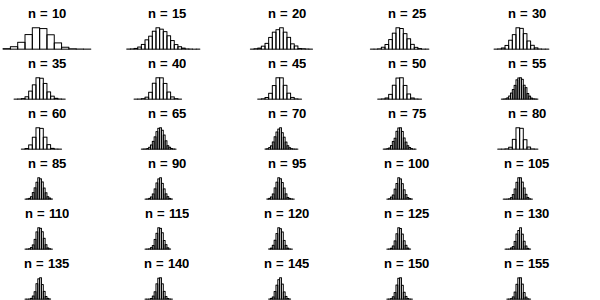
\includegraphics{images/samplingDist.png}
\item
  Using multiple cores to speed up computations

  In the previous example we generated the data on each iteration.
  This kind of simulation can be useful, but often you want to
  parallelize a function that processes data from a (potentially
  large) number of files. This is also easy to do using the parallel
  package in R. In the following example we count number of characters
  in all the text files in the texlive directory.

\begin{Shaded}
\begin{Highlighting}[]
\CommentTok{\#\# List the files to iterate over}
\NormalTok{textFiles\textless{}{-}}\StringTok{ }\KeywordTok{list.files}\NormalTok{(}\StringTok{"/usr/share/texlive/"}\NormalTok{,}
                       \DataTypeTok{recursive =} \OtherTok{TRUE}\NormalTok{,}
                       \DataTypeTok{pattern =} \StringTok{"}\CharTok{\textbackslash{}\textbackslash{}}\StringTok{.txt$|}\CharTok{\textbackslash{}\textbackslash{}}\StringTok{.tex$"}\NormalTok{,}
                       \DataTypeTok{full.names =} \OtherTok{TRUE}\NormalTok{)}

\CommentTok{\#\# function for counting characters (}\AlertTok{NOTE}\CommentTok{: this example isn\textquotesingle{}t realistic {-}{-} it}
\CommentTok{\#\# would be better to use the unix "wc" utility if you were doing this}
\CommentTok{\#\# in real life...)}
\NormalTok{countChars \textless{}{-}}\StringTok{  }\ControlFlowTok{function}\NormalTok{(x) \{}
  \KeywordTok{sum}\NormalTok{(}\KeywordTok{nchar}\NormalTok{(}\KeywordTok{readLines}\NormalTok{(x, }\DataTypeTok{warn =} \OtherTok{FALSE}\NormalTok{), }\DataTypeTok{type =} \StringTok{"width"}\NormalTok{))}
\NormalTok{\}}
\end{Highlighting}
\end{Shaded}

  We have \VERB|\KeywordTok{length}\NormalTok{(textFiles)}|
  text files to process. We can do this using a single core:

\begin{Shaded}
\begin{Highlighting}[]
\KeywordTok{system.time}\NormalTok{(nchars \textless{}{-}}\StringTok{ }\KeywordTok{unlist}\NormalTok{(}\KeywordTok{lapply}\NormalTok{(textFiles, countChars)))}
\end{Highlighting}
\end{Shaded}

  but this is too slow. We can do the computation more quickly using
  multiple cores:

\begin{Shaded}
\begin{Highlighting}[]
\KeywordTok{system.time}\NormalTok{(nchars \textless{}{-}}\StringTok{ }\KeywordTok{unlist}\NormalTok{(}\KeywordTok{mclapply}\NormalTok{(textFiles, countChars, }\DataTypeTok{mc.cores =} \DecValTok{7}\NormalTok{)))}
\end{Highlighting}
\end{Shaded}

  and calculate the total number of characters in the text files by
  summing over the result

\begin{Shaded}
\begin{Highlighting}[]
\KeywordTok{sum}\NormalTok{(nchars, }\DataTypeTok{na.rm =} \OtherTok{TRUE}\NormalTok{)}
\end{Highlighting}
\end{Shaded}

  For more details and examples using the parallel package, refer to
  the \href{https://stat.ethz.ch/R-manual/R-devel/library/parallel/doc/parallel.pdf}{parallel package
  documentation}
  or run \texttt{help(package\ =\ "parallel")} at the R prompt. For other ways
  of running computations in parallel refer to the \href{http://cran.r-project.org/web/views/HighPerformanceComputing.html}{HPC task
  view}.
\end{enumerate}

\hypertarget{python}{%
\subsection{Python}\label{python}}

Running computations in parallel on multiple cores is often an effective
way to speed up computations. This can be useful when we want to iterate
over a set of inputs, e.g., applying a function to each of a set of
files. In this example we count the number of characters in all the
files under the texlive directory.

\begin{Shaded}
\begin{Highlighting}[]
\ImportTok{import}\NormalTok{ os}
\ImportTok{import}\NormalTok{ fnmatch}
\NormalTok{textFiles }\OperatorTok{=}\NormalTok{ []}
\ControlFlowTok{for}\NormalTok{ root, dirnames, filenames }\KeywordTok{in}\NormalTok{ os.walk(}\StringTok{\textquotesingle{}/usr/share/texlive\textquotesingle{}}\NormalTok{):}
    \ControlFlowTok{for}\NormalTok{ filename }\KeywordTok{in}\NormalTok{ fnmatch.}\BuiltInTok{filter}\NormalTok{(filenames, }\StringTok{\textquotesingle{}*.tex\textquotesingle{}}\NormalTok{) }\OperatorTok{+}\NormalTok{ fnmatch.}\BuiltInTok{filter}\NormalTok{(filenames, }\StringTok{"*.txt"}\NormalTok{):}
\NormalTok{        textFiles.append(os.path.join(root, filename))}
\end{Highlighting}
\end{Shaded}

We have \texttt{len(textFiles)\ 2080} text files to process. We can do this using a
single core:

\begin{Shaded}
\begin{Highlighting}[]
\ImportTok{import}\NormalTok{ time}
\NormalTok{start }\OperatorTok{=}\NormalTok{ time.time()}

\NormalTok{num\_chars }\OperatorTok{=} \DecValTok{0}
\ControlFlowTok{for}\NormalTok{ fname }\KeywordTok{in}\NormalTok{ textFiles:}
    \ControlFlowTok{try}\NormalTok{:}
        \ControlFlowTok{with} \BuiltInTok{open}\NormalTok{(fname, }\StringTok{\textquotesingle{}r\textquotesingle{}}\NormalTok{) }\ImportTok{as}\NormalTok{ f:}
            \ControlFlowTok{for}\NormalTok{ line }\KeywordTok{in}\NormalTok{ f:}
\NormalTok{                num\_chars }\OperatorTok{+=} \BuiltInTok{len}\NormalTok{(line)}
    \ControlFlowTok{except}\NormalTok{:}
        \ControlFlowTok{pass}

\NormalTok{stop }\OperatorTok{=}\NormalTok{ time.time()}
\end{Highlighting}
\end{Shaded}

It takes around \texttt{print(stop\ -\ start)\ 1.27} seconds to
count the characters in these files, which is aleady pretty fast. But,
for even more speed we can use the \texttt{multiprocessing} library to perform
the operation using multiple cores:

\begin{Shaded}
\begin{Highlighting}[]
\ImportTok{import}\NormalTok{ multiprocessing}

\KeywordTok{def}\NormalTok{ f(fname):}
\NormalTok{    num\_chars }\OperatorTok{=}\NormalTok{ []}
    \ControlFlowTok{try}\NormalTok{:}
        \ControlFlowTok{with} \BuiltInTok{open}\NormalTok{(fname, }\StringTok{\textquotesingle{}r\textquotesingle{}}\NormalTok{) }\ImportTok{as}\NormalTok{ this\_file:}
            \ControlFlowTok{for}\NormalTok{ line }\KeywordTok{in}\NormalTok{ this\_file:}
\NormalTok{                num\_chars.append(}\BuiltInTok{len}\NormalTok{(line))}
    \ControlFlowTok{except}\NormalTok{:}
        \ControlFlowTok{pass}
    \ControlFlowTok{return} \BuiltInTok{sum}\NormalTok{(num\_chars)}

\NormalTok{start }\OperatorTok{=}\NormalTok{ time.time()}

\NormalTok{pool }\OperatorTok{=}\NormalTok{ multiprocessing.Pool(}\DecValTok{7}\NormalTok{)}
\NormalTok{nchar }\OperatorTok{=}\NormalTok{ pool.}\BuiltInTok{map}\NormalTok{(f, textFiles)}
\NormalTok{pool.close()}
\NormalTok{pool.join()}

\NormalTok{end }\OperatorTok{=}\NormalTok{ time.time()}
\end{Highlighting}
\end{Shaded}

which reduces the time to \texttt{print(end\ -\ start)\ 0.33} seconds.

\hypertarget{other-languages}{%
\subsection{Other languages}\label{other-languages}}

Using multiple CPU cores in Stata, Matlab and SAS does not require
explicit activation -- many functions will automatically use multiple
cores if available. For Matlab user-written code can also take advantage
of multiple CPUs using the \texttt{parfor} command. Python uses can run
multiple processes using the
\href{https://docs.python.org/2/library/multiprocessing.html}{multiprocessing}
library.

\hypertarget{batch-jobs}{%
\chapter{Batch Jobs}\label{batch-jobs}}

The RCE provides access to \emph{batch nodes}, a cluster of many computers.
The batch nodes are good for jobs will run for a long time, and for
groups of very similar jobs (e.g., simulations where a number of
parameters are varied).

Running jobs on the batch nodes is somewhat more complicated than
running \emph{interactive jobs} on the RCE. The main access points are two
\emph{command line} programs, \texttt{condor\_submit\_util} and \texttt{condor\_submit}. In
this tutorial we focus on writing simple submit files and submitting
them with \texttt{condor\_submit}. For more details on automatically generating
and submitting using \texttt{condor\_submit\_util} refer to the main \href{http://projects.iq.harvard.edu/rce/book/batch-processing-basics}{RCE batch
job
documentation}.

\hypertarget{preparing-a-batch-submission}{%
\section{Preparing a batch submission}\label{preparing-a-batch-submission}}

In practical terms, running in `batch' means that you will not be able
to interact with the running process. This means that all the
information your program needs to successfully complete needs to be
specified ahead of time. You can pass arguments to your process so that
each job gets different inputs, but the script must process these
arguments and do the right thing without further instruction.

When you submit a job to the batch processing system each process will
generate output and (perhaps) errors. It is usually a good idea to make
a sub-folder to store these results. Thus your project folder should
contain at least the following:

\begin{itemize}
\tightlist
\item
  script or program to run
\item
  submit file
\item
  output directory
\end{itemize}

When preparing your job for batch submission you usually need to figure
out how to split up the computation, (with one piece going to each
process), and how to tell each process which piece it is responsible
for. The examples below illustrate how to do this.

\hypertarget{submit-file-overview}{%
\section{Submit file overview}\label{submit-file-overview}}

In order to run jobs in parallel on the batch nodes you need to create a
\texttt{submit\ file} that describes the process to be run on each node. If
creating these files by hand you may use any text editor (e.g., \texttt{gedit},
accessible though the \texttt{Applications\ -\/-\textgreater{}\ Accessories} menu on the RCE).

The submit file template below includes all required elements. (Note
that this file is a template only -- see the next section for working
examples.)

\begin{verbatim}
# Universe whould always be 'vanilla'. This line MUST be
#included in your submit file, exactly as shown below.
Universe = vanilla

# The following arguments are _optional_. If included
# they are used to specify the requirements for the
# submission.
request_cpus = 1
request_disk = 4GB
request_memory = 4GB

# Enter the path to the program you wish to run.
# The default runs the R program. To run another
# program just change '/user/local/bin/R' to the
# path to the program you want to run. For example,
# to run Stata set Executable to '/usr/local/bin/stata'.
Executable = /usr/local/bin/R

# Specify any arguments you want to pass to the executable.
Arguments = --no-save --no-restore --slave

# Specify the relative path to the input file (if any). If you
# are using R this should be your R script. If you are using
# Stata this should be your do file.
input = example.R

# Specify where to output any results printed by your program.
output = output/out.$(Process)
# Specify where to save any errors returned by your program.
error = output/error.$(Process)
# Specify where to save the log file.
Log = output/log
# Enter the number of processes to request. This should
# always be the last part of your submit file.
Queue 10
\end{verbatim}

This submit file instructs the scheduler to request 10 nodes
(\texttt{Queue\ 10}), start R on each one (\texttt{Executable\ =\ /usr/local/bin/R}),
run the code in example.R (\texttt{input\ =\ example.R}), write the output to
files named out.0 -- out.9 in the output folder
(\texttt{output\ =\ output/out.\$(Process)}), write any errors to files named
out.0 -- out.9 in the output folder (\texttt{error\ =\ output/error.\$(Process)}),
and write a log file in the output folder (\texttt{Log\ =\ output/log}). Each of
the 10 requested nodes must be able to provide at least one cpu
(\texttt{request\_cpus\ =\ 1}), four Gb of disk space (\texttt{request\_disk\ =\ 4GB}) and
four Gb of memory (\texttt{request\_memory\ =\ 4GB}).

The elements included in the submit file template above should be
suffucient for most jobs. You can \href{template.submit}{download this submit file
template} and modify it to suit your needs. For a
complete description of the Condor submit file syntax, including less
commonly used elements not described here refer to the \href{https://htcondor.readthedocs.io/en/v8_8_3/man-pages/condor_submit.html}{official
documentation}.

\hypertarget{monitoring-and-managing}{%
\section{Monitoring and managing}\label{monitoring-and-managing}}

After submitting the jobs we may wish to monitor them, e.g.~to check if
they are running. You can do this by running \texttt{condor\_q\ \textless{}your\_user\_name\textgreater{}}
in a terminal. If this returns nothing then you have no jobs in the
queue. Otherwise you will see information for each request in the queue
which will look something like this:

\begin{verbatim}
-- Schedd: HMDC.batch@rce6-5.hmdc.harvard.edu : <10.0.0.10:9619?sock=7858_e19e_247>
 ID      OWNER            SUBMITTED     RUN_TIME ST PRI SIZE CMD
 200.0   izahn           4/27 11:45   0+00:00:04 R  0   0.0  R --no-save --no-r
 200.1   izahn           4/27 11:45   0+00:00:04 R  0   0.0  R --no-save --no-r
 200.2   izahn           4/27 11:45   0+00:00:04 R  0   0.0  R --no-save --no-r
 200.3   izahn           4/27 11:45   0+00:00:04 R  0   0.0  R --no-save --no-r
 200.4   izahn           4/27 11:45   0+00:00:04 R  0   0.0  R --no-save --no-r
 200.5   izahn           4/27 11:45   0+00:00:04 R  0   0.0  R --no-save --no-r
 200.6   izahn           4/27 11:45   0+00:00:04 R  0   0.0  R --no-save --no-r
 200.7   izahn           4/27 11:45   0+00:00:04 R  0   0.0  R --no-save --no-r
 200.8   izahn           4/27 11:45   0+00:00:04 R  0   0.0  R --no-save --no-r
 200.9   izahn           4/27 11:45   0+00:00:04 R  0   0.0  R --no-save --no-r
 200.10  izahn           4/27 11:45   0+00:00:04 R  0   0.0  R --no-save --no-r
 200.11  izahn           4/27 11:45   0+00:00:04 R  0   0.0  R --no-save --no-r
 200.12  izahn           4/27 11:45   0+00:00:04 R  0   0.0  R --no-save --no-r
\end{verbatim}

Perhaps the most important information returned by \texttt{condor\_q} is the
program status (the \textbf{ST} column). Status \textbf{I} means your job is in
the queue but has not yet started running, \textbf{R} means the job is
currently running, and \textbf{H} means the job is on hold. If you job is on
hold you can get more information about what the problem might be by
running \texttt{condor\_q\ -hold}.

You will know your job is finished when it is no longer listed in the
\texttt{condor\_q} output. When it finishes you can examine the output and/or
error files to see if the program exited successfully.

If you would like to remove a batch job from the queue you may do so
using \texttt{condor\_rm}. For example \texttt{condor\_rm\ 200} will remove the jobs
listed above.

For more details on monitoring and manageing your batch jobs please
refer to
\url{http://projects.iq.harvard.edu/rce/book/checking-your-process-status}

\hypertarget{batch-job-examples}{%
\chapter{Batch Job Examples}\label{batch-job-examples}}

RCE users come from a variety of backgrounds and different people are
more proficient with different software packages. Feel free to skip to
the batch examples using the software you are most comfortable with:

\hypertarget{r-1}{%
\section{R}\label{r-1}}

\hypertarget{power-simulation}{%
\subsection{Power simulation}\label{power-simulation}}

The simplest kind of batch job is one for which you just want to run the
same code multiple times, without varying any parameters. For example,
suppose that we wish to run a power simulation for a t.test with unequal
group sizes.

\begin{enumerate}
\def\labelenumi{\arabic{enumi}.}
\item
  Simulation script

  The first step is to write a script or program to carry out the
  desired computation. The R script below simulates distributions with
  a specified mean difference, performs two-sample t-tests on the
  difference, and calculates the proportion of significant tests.

\begin{Shaded}
\begin{Highlighting}[]
\CommentTok{\#\# function to simulate data and perform a t.test}
\NormalTok{sim.ttest \textless{}{-}}\StringTok{ }\ControlFlowTok{function}\NormalTok{(mu1, mu2, sd, n1, n2) \{}
\NormalTok{    d \textless{}{-}}\StringTok{ }\KeywordTok{data.frame}\NormalTok{(}\DataTypeTok{x =} \KeywordTok{c}\NormalTok{(}\KeywordTok{rep}\NormalTok{(}\StringTok{"group1"}\NormalTok{, n1), }\KeywordTok{rep}\NormalTok{(}\StringTok{"group2"}\NormalTok{, n2)),}
                    \DataTypeTok{y =} \KeywordTok{c}\NormalTok{(}\KeywordTok{rnorm}\NormalTok{(n1, }\DataTypeTok{mean =}\NormalTok{ mu1, }\DataTypeTok{sd =}\NormalTok{ sd),}
                          \KeywordTok{rnorm}\NormalTok{(n2, }\DataTypeTok{mean =}\NormalTok{ mu2, }\DataTypeTok{sd =}\NormalTok{ sd)))}
    \KeywordTok{return}\NormalTok{(}\KeywordTok{t.test}\NormalTok{(y }\OperatorTok{\textasciitilde{}}\StringTok{ }\NormalTok{x, }\DataTypeTok{data =}\NormalTok{ d)}\OperatorTok{$}\NormalTok{p.value)}
\NormalTok{\}}

\CommentTok{\#\#  run the function 10,000 times}
\NormalTok{p \textless{}{-}}\StringTok{ }\KeywordTok{replicate}\NormalTok{(}\DecValTok{10000}\NormalTok{,}
               \KeywordTok{sim.ttest}\NormalTok{(}\DataTypeTok{mu1 =} \DecValTok{1}\NormalTok{,}
                         \DataTypeTok{mu2 =} \FloatTok{1.3}\NormalTok{,}
                         \DataTypeTok{sd =} \DecValTok{1}\NormalTok{,}
                         \DataTypeTok{n1 =} \DecValTok{50}\NormalTok{,}
                         \DataTypeTok{n2 =} \DecValTok{150}\NormalTok{))}
\CommentTok{\#\# calculate the proportion of significant tests}
\KeywordTok{cat}\NormalTok{(}\KeywordTok{length}\NormalTok{(p[p }\OperatorTok{\textless{}}\StringTok{ }\FloatTok{.05}\NormalTok{])}\OperatorTok{/}\KeywordTok{length}\NormalTok{(p))}
\end{Highlighting}
\end{Shaded}
\item
  Submit file

  If we want to run this function one million times it may take a
  while, especially if our computer is an older less powerful model.
  So let's run it on 100 separate machines (each one will simulate the
  test 10000 times). To do that we need, in addition to the R script
  above, a submit file to request resources and run the computation.

\begin{verbatim}
# Universe whould always be 'vanilla'. This line MUST be
#included in your submit file, exactly as shown below.
Universe = vanilla

# Enter the path to the R program.
Executable = /usr/local/bin/R

# Specify any arguments you want to pass to the executable.
# Here we pass arguments to make R not save or restore workspaces,
# and to run as quietly as possible.
Arguments = --no-save --no-restore --slave

# Specify the relative path to the input file
input = power.R

# Specify where to output any results printed by your program.
output = output/out.$(Process)
# Specify where to save any errors returned by your program.
error = output/error.$(Process)
# Specify where to save the log file.
Log = output/log

# Enter the number of processes to request.
# This section should always come last.
Queue 100
\end{verbatim}

  Now that we have our script and the submit file we can run submit
  the job as follows:

  \begin{enumerate}
  \def\labelenumii{\arabic{enumii}.}
  \tightlist
  \item
    make a project folder for this run if it doesn't exist
  \item
    save the R script (as power.R) and the submit file (as
    power.submit) in the project folder
  \item
    make a sub folder named \texttt{output}
  \item
    open a terminal and \texttt{cd} to the project folder
  \item
    run \texttt{condor\_submit\ power.submit} to submit the jobs to the
    cluster
  \end{enumerate}
\item
  Aggregating results

  When your batch job is finished you are usually left with multiple
  output files that need to be aggregated. In the case of our
  simulation example, we have files \texttt{output/out.0\ -\/-\ output/out99},
  each of which contains a single number representing the proportion
  of significant tests. We can aggregate them with a simple R script,
  like this:

\begin{Shaded}
\begin{Highlighting}[]
\CommentTok{\#\# list all output files in the output directory}
\NormalTok{output\_files \textless{}{-}}\StringTok{ }\KeywordTok{list.files}\NormalTok{(}\StringTok{"output"}\NormalTok{,}
                           \DataTypeTok{pattern =} \StringTok{"\^{}out}\CharTok{\textbackslash{}\textbackslash{}}\StringTok{.[0{-}9]+$"}\NormalTok{,}
                           \DataTypeTok{full.names=}\OtherTok{TRUE}\NormalTok{)}

\CommentTok{\#\# read each file, convert it to a number, and take the average}
\KeywordTok{mean}\NormalTok{(}\KeywordTok{as.double}\NormalTok{(}\KeywordTok{sapply}\NormalTok{(}
\NormalTok{                      output\_files,}
\NormalTok{                      readLines,}
                      \DataTypeTok{warn =} \OtherTok{FALSE}\NormalTok{)))}
\end{Highlighting}
\end{Shaded}
\item
  Try it yourself!

  Download the \href{examples_R/power1.zip}{power simulation example
  files}, to the RCE, extract the zip file and
  running \texttt{condor\_submit\ power.submit} in the \texttt{power1} directory.
\end{enumerate}

\hypertarget{varying-parameters}{%
\subsection{Varying parameters}\label{varying-parameters}}

The previous example was relatively simple, because we wanted to run
exactly the same code on all 100 nodes. Often however you want each node
to do something slightly different. For example, we may wish to vary the
sample size from 100 -- 500 in increments of 10, to see how power
changes as a function of that parameter. In that case we need to pass
some additional information to each process, telling it which parameter
space it is responsible for.

As it turns out, we almost already know how to do that: if you you look
closely at the submit file in the previous example you will notice that
we used \texttt{\$(Process)} to append the process number to the output and
error files.

\begin{enumerate}
\def\labelenumi{\arabic{enumi}.}
\item
  Submit file passing process as an argument

  We can use the \texttt{\$(Process)} macro to pass information to our
  program, like this:

\begin{verbatim}
# Universe whould always be 'vanilla'. This line MUST be
#included in your submit file, exactly as shown below.
Universe = vanilla

# Enter the path to the R program.
Executable = /usr/local/bin/R

# Specify any arguments you want to pass to the executable
# to make r not save or restore workspaces, and to
# run as quietly as possible
Arguments = --no-save --no-restore --slave --args $(Process)

# Specify the relative path to the input file
input = power.R

# Specify where to save any errors returned by your program.
error = output/error.$(Process)

Log = log.txt
# Enter the number of processes to request.
Queue 40
\end{verbatim}

  Notice that we used \texttt{-\/-args\ \$(Process)} to pass the process number
  to the R program. \texttt{\$(Process)} will be an integer starting from \texttt{0}.
\item
  Argument processing

  Next we need to 1) retrieve the process number in our R program
  and 2) map it to the parameter space. We can retrieve the arguments
  in R like this:

\begin{Shaded}
\begin{Highlighting}[]
\CommentTok{\#\# retrieve arguments passed from the command line.}
\NormalTok{process \textless{}{-}}\StringTok{ }\KeywordTok{as.integer}\NormalTok{(}\KeywordTok{as.character}\NormalTok{(}\KeywordTok{commandArgs}\NormalTok{(}\DataTypeTok{trailingOnly =} \OtherTok{TRUE}\NormalTok{)))}
\end{Highlighting}
\end{Shaded}

  We now have a variable in R that tells us which process we are. Now
  we need to map that to our parameter space; recall that we want to
  test sample sizes from 100 to 500, so we need to map \texttt{process\ 0} to
  \texttt{n\ =\ 100}, \texttt{process\ 1} to \texttt{n\ =\ 110}, \texttt{process\ 2} to \texttt{n\ =\ 120} and so
  on:

\begin{Shaded}
\begin{Highlighting}[]
\CommentTok{\#\# map process to sample size parameter.}
\NormalTok{n \textless{}{-}}\StringTok{ }\NormalTok{(process }\OperatorTok{+}\StringTok{ }\DecValTok{100}\NormalTok{) }\OperatorTok{+}\StringTok{ }\NormalTok{(process}\OperatorTok{*}\DecValTok{10} \OperatorTok{{-}}\StringTok{ }\NormalTok{process)}
\end{Highlighting}
\end{Shaded}

  There is one additional complication we need to handle: in the
  previous example we did need to keep track of the parameters used by
  each process because the parameters did not vary. Now that they do,
  it would be nice if we had output that recorded the value of the
  varying parameter as well as the result. We could of course just
  print the \texttt{n} parameter we calculated from the process number along
  with the result, but it will be easier to combine the outputs if we
  write them to a machine-readable format (e.g., a
  comma-separated-values file). You may have noticed that in the
  submit file above I omitted the \texttt{output} directive: that is because
  we are going to explicitly save the results in the R script, so we
  don't need the batch scheduler to save those output files for us.

  Now we can set up the simulation as before, passing the \texttt{n}
  calculated above into our simulation function, writing the results
  to files.

\begin{Shaded}
\begin{Highlighting}[]
  \CommentTok{\#\# function to simulate data and perform a t.test}
\NormalTok{  sim.ttest \textless{}{-}}\StringTok{ }\ControlFlowTok{function}\NormalTok{(mu1, mu2, sd, n1, n2) \{}
\NormalTok{      d \textless{}{-}}\StringTok{ }\KeywordTok{data.frame}\NormalTok{(}\DataTypeTok{x =} \KeywordTok{c}\NormalTok{(}\KeywordTok{rep}\NormalTok{(}\StringTok{"group1"}\NormalTok{, n1), }\KeywordTok{rep}\NormalTok{(}\StringTok{"group2"}\NormalTok{, n2)),}
                      \DataTypeTok{y =} \KeywordTok{c}\NormalTok{(}\KeywordTok{rnorm}\NormalTok{(n1, }\DataTypeTok{mean =}\NormalTok{ mu1, }\DataTypeTok{sd =}\NormalTok{ sd),}
                            \KeywordTok{rnorm}\NormalTok{(n2, }\DataTypeTok{mean =}\NormalTok{ mu2, }\DataTypeTok{sd =}\NormalTok{ sd)))}
      \KeywordTok{return}\NormalTok{(}\KeywordTok{t.test}\NormalTok{(y }\OperatorTok{\textasciitilde{}}\StringTok{ }\NormalTok{x, }\DataTypeTok{data =}\NormalTok{ d)}\OperatorTok{$}\NormalTok{p.value)}
\NormalTok{  \}}

  \CommentTok{\#\#  run the function 10,000 times}
\NormalTok{  p \textless{}{-}}\StringTok{ }\KeywordTok{replicate}\NormalTok{(}\DecValTok{10000}\NormalTok{,}
                 \KeywordTok{sim.ttest}\NormalTok{(}\DataTypeTok{mu1 =} \DecValTok{1}\NormalTok{,}
                           \DataTypeTok{mu2 =} \FloatTok{1.3}\NormalTok{,}
                           \DataTypeTok{sd =} \DecValTok{1}\NormalTok{,}
                           \DataTypeTok{n1 =}\NormalTok{ n,}
                           \DataTypeTok{n2 =}\NormalTok{ n))}
\KeywordTok{write.csv}\NormalTok{(}\KeywordTok{data.frame}\NormalTok{(}\DataTypeTok{n =}\NormalTok{ n, }\DataTypeTok{power =} \KeywordTok{length}\NormalTok{(p[p }\OperatorTok{\textless{}}\StringTok{ }\FloatTok{.05}\NormalTok{])}\OperatorTok{/}\KeywordTok{length}\NormalTok{(p)),}
          \DataTypeTok{row.names =} \OtherTok{FALSE}\NormalTok{,}
          \DataTypeTok{file =} \KeywordTok{paste0}\NormalTok{(}\StringTok{"output/out"}\NormalTok{, process, }\StringTok{".csv"}\NormalTok{))}
\end{Highlighting}
\end{Shaded}

  Now we have all the required elements to submit out job, and can do
  so using \texttt{condor\_submit} as before.
\item
  Aggregating results

  Each of our 40 processes produced a file in the \texttt{output} directory
  name \texttt{out\textless{}process\textgreater{}csv}; our next task is to aggregate these results.
  The R script below reads each of these files, joins them together
  into a single data.frame, and plots the result.

\begin{Shaded}
\begin{Highlighting}[]
\CommentTok{\#\# list all output files in the output directory}
\NormalTok{output\_files \textless{}{-}}\StringTok{ }\KeywordTok{list.files}\NormalTok{(}\StringTok{"output"}\NormalTok{,}
                           \DataTypeTok{pattern =} \StringTok{"\^{}out[0{-}9]+}\CharTok{\textbackslash{}\textbackslash{}}\StringTok{.csv$"}\NormalTok{,}
                           \DataTypeTok{full.names=}\OtherTok{TRUE}\NormalTok{)}

\CommentTok{\#\# read each file and append them}
\NormalTok{results \textless{}{-}}\StringTok{ }\KeywordTok{do.call}\NormalTok{(rbind, }\KeywordTok{lapply}\NormalTok{(output\_files, read.csv))}

\CommentTok{\#\# plot}
\KeywordTok{plot}\NormalTok{(results)}
\KeywordTok{abline}\NormalTok{(}\DataTypeTok{h =} \FloatTok{0.8}\NormalTok{)}
\end{Highlighting}
\end{Shaded}

  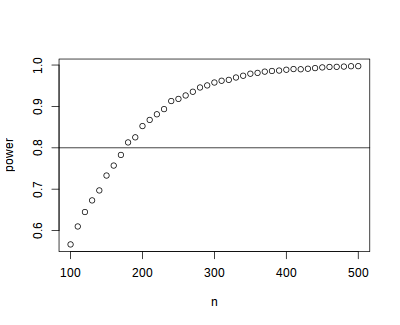
\includegraphics{images/powerDist.png}
\item
  Try it yourself!

  Download the \href{examples_R/power2.zip}{power simulation example files}, to the RCE, extract the zip file, and
  run the example by calling \texttt{condor\_submit\ power.submit} from the
  \texttt{power2} directory.
\end{enumerate}

\hypertarget{python-1}{%
\section{Python}\label{python-1}}

\hypertarget{power-simulation-1}{%
\subsection{Power simulation}\label{power-simulation-1}}

The simplest kind of batch job is one for which you just want to run the
same code multiple times, without varying any parameters. For example,
suppose that we wish to run a power simulation for a t-test with unequal
group sizes.

\begin{enumerate}
\def\labelenumi{\arabic{enumi}.}
\item
  Simulation script

  The first step is to write a script or program to carry out the
  desired computation. The python script below simulates distributions
  with a specified mean difference, performs two-sample t-tests on the
  difference, and calculates the proportion of significant tests.

\begin{Shaded}
\begin{Highlighting}[]
\ImportTok{import}\NormalTok{ numpy }\ImportTok{as}\NormalTok{ np}
\ImportTok{from}\NormalTok{ scipy }\ImportTok{import}\NormalTok{ stats}

\CommentTok{\#\# function to simulate data and perform a t.test}
\KeywordTok{def}\NormalTok{ sim\_ttest(mu1, mu2, sd, n1, n2):}
\NormalTok{    x }\OperatorTok{=}\NormalTok{ stats.norm.rvs(loc }\OperatorTok{=}\NormalTok{ mu1, scale }\OperatorTok{=}\NormalTok{ sd, size }\OperatorTok{=}\NormalTok{ n1)}
\NormalTok{    y }\OperatorTok{=}\NormalTok{ stats.norm.rvs(loc }\OperatorTok{=}\NormalTok{ mu2, scale }\OperatorTok{=}\NormalTok{ sd, size }\OperatorTok{=}\NormalTok{ n2)}
    \ControlFlowTok{return}\NormalTok{(stats.ttest\_ind(x, y)[}\DecValTok{1}\NormalTok{])}

\CommentTok{\#\#  run the function 10,000 times}
\NormalTok{nsims }\OperatorTok{=} \DecValTok{10000}
\NormalTok{p }\OperatorTok{=}\NormalTok{ [sim\_ttest(}\DecValTok{1}\NormalTok{, }\FloatTok{1.3}\NormalTok{, }\DecValTok{1}\NormalTok{, }\DecValTok{50}\NormalTok{, }\DecValTok{150}\NormalTok{)  }\ControlFlowTok{for}\NormalTok{ x }\KeywordTok{in} \BuiltInTok{range}\NormalTok{(nsims)]}
\CommentTok{\#\# calculate proportion of significant tests}
\BuiltInTok{print}\NormalTok{(}\BuiltInTok{len}\NormalTok{([x }\ControlFlowTok{for}\NormalTok{ x }\KeywordTok{in}\NormalTok{ p }\ControlFlowTok{if}\NormalTok{ x }\OperatorTok{\textless{}} \FloatTok{.05}\NormalTok{])}\OperatorTok{/}\NormalTok{nsims)}
\end{Highlighting}
\end{Shaded}
\item
  Submit file

  If we want to run this function one million times it may take a
  while, especially if our computer is an older less powerful model.
  So let's run it on 100 separate machines (each one will simulate the
  test 10000 times). To do that we need, in addition to the python
  script above, a submit file to request resources and run the
  computation.

\begin{verbatim}
# Universe whould always be 'vanilla'. This line MUST be
#included in your submit file, exactly as shown below.
Universe = vanilla

# Enter the path to the python program.
Executable = /usr/local/bin/python33

# Specify any arguments you want to pass to the executable.
# Here we pass arguments to make python not save or restore workspaces,
# and to run as quietly as possible.
Arguments = power.py

# Note that unlike R batch job submission we pass the python script in
# the Arguments section rather than in the "Input" section.
# Specify the relative path to the input file

# Specify where to output any results printed by your program.
output = output/out.$(Process)
# Specify where to save any errors returned by your program.
error = output/error.$(Process)
# Specify where to save the log file.
Log = output/log

# Enter the number of processes to request.
# This section should always come last.
Queue 100
\end{verbatim}

  Now that we have our script and the submit file we can run submit
  the job as follows:

  \begin{enumerate}
  \def\labelenumii{\arabic{enumii}.}
  \tightlist
  \item
    make a project folder for this run if it doesn't exist
  \item
    save the python script (as power.python) and the submit file (as
    power.submit) in the project folder
  \item
    make a sub folder named \texttt{output}
  \item
    open a terminal and \texttt{cd} to the project folder
  \item
    run \texttt{condor\_submit\ power.submit} to submit the jobs to the cluster
  \end{enumerate}
\item
  Aggregating results

  When your batch job is finished you are usually left with multiple
  output files that need to be aggregated. In the case of our
  simulation example, we have files \texttt{output/out.0\ -\/-\ output/out99},
  each of which contains a single number representing the proportion
  of significant tests. We can aggregate them with a simple python
  script, like this:

\begin{Shaded}
\begin{Highlighting}[]
\ImportTok{import}\NormalTok{ numpy }\ImportTok{as}\NormalTok{ np}
\ImportTok{import}\NormalTok{ glob}
\CommentTok{\#\# list all output files in the output directory}
\NormalTok{output\_files }\OperatorTok{=}\NormalTok{ glob.glob(}\StringTok{"output/out*"}\NormalTok{)}

\NormalTok{output\_values }\OperatorTok{=} \BuiltInTok{map}\NormalTok{(}\KeywordTok{lambda}\NormalTok{ f: np.}\BuiltInTok{float}\NormalTok{(}\BuiltInTok{open}\NormalTok{(f).read()), output\_files)}
\BuiltInTok{print}\NormalTok{(}\BuiltInTok{list}\NormalTok{(output\_values))}
\end{Highlighting}
\end{Shaded}
\item
  Try it yourself!

  Download the \href{examples_Python/power1.zip}{power simulation example
  files}, to the pythonCE, extract the zip
  file and running \texttt{condor\_submit\ power.submit} in the \texttt{power1}
  directory.
\end{enumerate}

\hypertarget{varying-parameters-1}{%
\subsection{Varying parameters}\label{varying-parameters-1}}

The previous example was relatively simple, because we wanted to run
exactly the same code on all 100 nodes. Often however you want each node
to do something slightly different. For example, we may wish to vary the
sample size from 100 -- 500 in increments of 10, to see how power
changes as a function of that parameter. In that case we need to pass
some additional information to each process, telling it which parameter
space it is responsible for.

As it turns out, we almost already know how to do that: if you you look
closely at the submit file in the previous example you will notice that
we used \texttt{\$(Process)} to append the process number to the output and
error files.

\begin{enumerate}
\def\labelenumi{\arabic{enumi}.}
\item
  Submit file passing process as an argument

  We can use the \texttt{\$(Process)} macro to pass information to our
  program, like this:

\begin{verbatim}
  # Universe whould always be 'vanilla'. This line MUST be
  #included in your submit file, exactly as shown below.
  Universe = vanilla

  # Enter the path to the python program.
  Executable = /usr/local/bin/python33

  # Specify any arguments you want to pass to the executable
  Arguments = power.py $(Process)

# Specify where to output any results printed by your program.
  output = output/out.$(Process)

  # Specify where to save any errors returned by your program.
  error = output/error.$(Process)

  Log = log.txt
  # Enter the number of processes to request.
  Queue 40
\end{verbatim}

  Notice that we used \texttt{-\/-args\ \$(Process)} to pass the process number
  to the python program. \texttt{\$(Process)} will be an integer starting from
  \texttt{0}.
\item
  Argument processing

  Next we need to 1) retrieve the process number in our python program
  and 2) map it to the parameter space. We can retrieve the arguments
  in python like this:

\begin{Shaded}
\begin{Highlighting}[]
\ImportTok{import}\NormalTok{ sys}
\CommentTok{\#\# retrieve arguments passed from the command line.}
\NormalTok{process }\OperatorTok{=} \BuiltInTok{int}\NormalTok{(sys.argv[}\DecValTok{1}\NormalTok{])}
\end{Highlighting}
\end{Shaded}

  We now have a variable in python that tells us which process we are.
  Now we need to map that to our parameter space; recall that we want
  to test sample sizes from 100 to 500, so we need to map \texttt{process\ 0}
  to \texttt{n\ =\ 100}, \texttt{process\ 1} to \texttt{n\ =\ 110}, \texttt{process\ 2} to \texttt{n\ =\ 120} and
  so on:

\begin{Shaded}
\begin{Highlighting}[]
\CommentTok{\#\# map process to sample size parameter.}
\NormalTok{n }\OperatorTok{=}\NormalTok{ (process }\OperatorTok{+} \DecValTok{100}\NormalTok{) }\OperatorTok{+}\NormalTok{ (process}\OperatorTok{*}\DecValTok{10} \OperatorTok{{-}}\NormalTok{ process)}
\end{Highlighting}
\end{Shaded}

  There is one additional complication we need to handle: in the
  previous example we did need to keep track of the parameters used by
  each process because the parameters did not vary. Now that they do,
  it would be nice if we had output that recorded the value of the
  varying parameter as well as the result. We could of course just
  print the \texttt{n} parameter we calculated from the process number along
  with the result, but it will be easier to combine the outputs if we
  write them to a machine-readable format (e.g., a
  comma-separated-values file). You may have noticed that in the
  submit file above I omitted the \texttt{output} directive: that is because
  we are going to explicitly save the results in the python script, so
  we don't need the batch scheduler to save those output files for us.

  Now we can set up the simulation as before, passing the \texttt{n}
  calculated above into our simulation function, writing the results
  to files.

\begin{Shaded}
\begin{Highlighting}[]
\CommentTok{\#\# function to simulate data and perform a t.test}
\ImportTok{import}\NormalTok{ numpy }\ImportTok{as}\NormalTok{ np}
\ImportTok{from}\NormalTok{ scipy }\ImportTok{import}\NormalTok{ stats}

\CommentTok{\#\# function to simulate data and perform a t.test}
\KeywordTok{def}\NormalTok{ sim\_ttest(mu1, mu2, sd, n1, n2):}
\NormalTok{    x }\OperatorTok{=}\NormalTok{ stats.norm.rvs(loc }\OperatorTok{=}\NormalTok{ mu1, scale }\OperatorTok{=}\NormalTok{ sd, size }\OperatorTok{=}\NormalTok{ n1)}
\NormalTok{    y }\OperatorTok{=}\NormalTok{ stats.norm.rvs(loc }\OperatorTok{=}\NormalTok{ mu2, scale }\OperatorTok{=}\NormalTok{ sd, size }\OperatorTok{=}\NormalTok{ n2)}
    \ControlFlowTok{return}\NormalTok{(stats.ttest\_ind(x, y)[}\DecValTok{1}\NormalTok{])}

\CommentTok{\#\#  run the function 10,000 times}
\NormalTok{nsims }\OperatorTok{=} \DecValTok{10000}
\NormalTok{p }\OperatorTok{=}\NormalTok{ [sim\_ttest(}\DecValTok{1}\NormalTok{, }\FloatTok{1.3}\NormalTok{, }\DecValTok{1}\NormalTok{, n, n)  }\ControlFlowTok{for}\NormalTok{ x }\KeywordTok{in} \BuiltInTok{range}\NormalTok{(nsims)]}
\BuiltInTok{print}\NormalTok{(}\BuiltInTok{len}\NormalTok{([x }\ControlFlowTok{for}\NormalTok{ x }\KeywordTok{in}\NormalTok{ p }\ControlFlowTok{if}\NormalTok{ x }\OperatorTok{\textless{}} \FloatTok{.05}\NormalTok{])}\OperatorTok{/}\NormalTok{nsims)}
\BuiltInTok{print}\NormalTok{(n)}
\end{Highlighting}
\end{Shaded}

  Now we have all the required elements to submit out job, and can do
  so using \texttt{condor\_submit} as before.
\item
  Aggregating results

  Each of our 40 processes produced a file in the \texttt{output} directory
  name \texttt{out\textless{}process\textgreater{}csv}; our next task is to aggregate these results.
  The python script below reads each of these files, joins them
  together into a single array, and plots the result.

\begin{Shaded}
\begin{Highlighting}[]
\ImportTok{import}\NormalTok{ numpy }\ImportTok{as}\NormalTok{ np}
\ImportTok{import}\NormalTok{ glob}
\ImportTok{import}\NormalTok{ matplotlib.pyplot }\ImportTok{as}\NormalTok{ plt}
\CommentTok{\#\# list all output files in the output directory}
\NormalTok{output\_files }\OperatorTok{=}\NormalTok{ glob.glob(}\StringTok{"output/out*"}\NormalTok{)}

\NormalTok{output\_values }\OperatorTok{=}\NormalTok{ np.array([x.split(}\StringTok{"}\CharTok{\textbackslash{}n}\StringTok{"}\NormalTok{)[:}\DecValTok{2}\NormalTok{]}
                          \ControlFlowTok{for}\NormalTok{ x }\KeywordTok{in}\NormalTok{ [}\BuiltInTok{open}\NormalTok{(f).read() }\ControlFlowTok{for}\NormalTok{ f }\KeywordTok{in}\NormalTok{ output\_files]],}
\NormalTok{                         dtype }\OperatorTok{=} \StringTok{"float"}\NormalTok{)}

\NormalTok{plt.plot(}\BuiltInTok{list}\NormalTok{(output\_values[:, }\DecValTok{1}\NormalTok{]), }\BuiltInTok{list}\NormalTok{(output\_values[:, }\DecValTok{0}\NormalTok{]), }\StringTok{"bo"}\NormalTok{)}
\NormalTok{plt.xlabel(}\StringTok{"Sample Size"}\NormalTok{)}
\NormalTok{plt.ylabel(}\StringTok{"Power"}\NormalTok{)}
\NormalTok{plt.savefig(}\StringTok{"power.png"}\NormalTok{)}
\end{Highlighting}
\end{Shaded}

  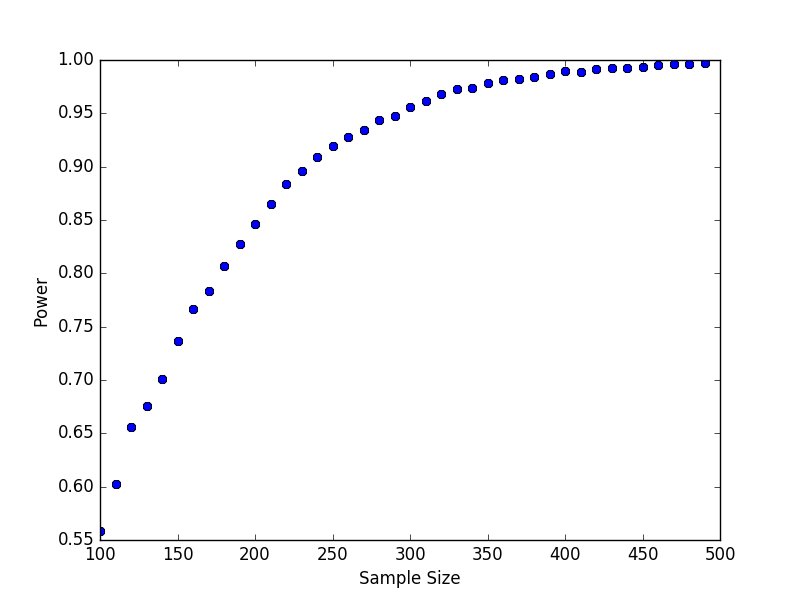
\includegraphics{images/python_powerDist.png}
\item
  Try it yourself!

  Download the \href{examples_Python/power2.zip}{power simulation example files}, to the pythonCE, extract the zip
  file, and run the example by calling \texttt{condor\_submit\ power.submit}
  from the \texttt{power2} directory.
\end{enumerate}

\hypertarget{stata}{%
\section{Stata}\label{stata}}

\begin{verbatim}
In this example we use the batch system to bootstrap a distribution of
means. Each process will calculate the mean for a single bootstrap
sample and save the result. Since we need to give the output files
unique names we will pass the batch process number to Stata and use it
to construct the file names.
\end{verbatim}

\begin{enumerate}
\def\labelenumi{\arabic{enumi}.}
\item
  Bootstrap do-file

  To use the batch system we need to write a do-file that does the
  calculation without further user input. The do-file below reads a Stata
  data set, sets a seed for random number generation, samples (with
  replacement) from the data, calculates the average value of the sampled
  data, and saves the result.

\begin{Shaded}
\begin{Highlighting}[]
\KeywordTok{set} \KeywordTok{more} \KeywordTok{off}

\CommentTok{// collect the arguments passed by submit file}
\KeywordTok{args}\NormalTok{ process}

\CommentTok{// load the dataset}
\KeywordTok{use} \StringTok{"mydata"}\NormalTok{, }\KeywordTok{clear}

\CommentTok{// set seed (shouldn\textquotesingle{}t have to do this, but stata\textquotesingle{}s}
\CommentTok{// random bsample defaults to the same seed each time).}
\CommentTok{// we nee to find a better way to do this.}
\KeywordTok{set} \DecValTok{seed} \OtherTok{\textasciigrave{}process\textquotesingle{}}

\CommentTok{// sample with replacement}
\KeywordTok{bsample}\NormalTok{, }\KeywordTok{cluster}\NormalTok{(id) idcluster(newid)}

\CommentTok{// calculate the mean and standard deviation}
\KeywordTok{collapse}\NormalTok{ (}\KeywordTok{mean}\NormalTok{) mean\_myvar = myvar (}\FunctionTok{sd}\NormalTok{) sd\_myvar = myvar}

\CommentTok{// save the result, appending the process number to the file name}
\KeywordTok{save} \StringTok{"output/output\_\textasciigrave{}process\textquotesingle{}.dta"}\NormalTok{, }\KeywordTok{replace}
\end{Highlighting}
\end{Shaded}

  Note the use of \texttt{args\ process}, which retrieves the value of the process
  argument. The argument itself is specified in the \texttt{.submit} file (see
  below).
\item
  Submit file

  The Stata code in the example above draws one bootstrap sample and
  calculates the mean. If we want to do this 1,000 times we could write a
  loop, but each iteration would be done sequentially. We can carry out
  this operation faster by running it simultaneously on hundreds of
  machines. We just need a \texttt{.submit} file like the one below:

\begin{verbatim}
# Universe whould always be 'vanilla'. This line MUST be
#included in your submit file, exactly as shown below.
Universe = vanilla

# Enter the path to the Stata program.
Executable = /usr/local/bin/stata-mp

# Specify any arguments you want to pass to the executable.
# Here we pass arguments to make Stata run the bootstrap.do
# file. We also pass the process number, which will be used
# to append the process number to the output files.
Arguments = -q do bootstrap.do $(Process)

# Specify where to output any results printed by your program.
output = output/bootstrap$(Process).out
# Specify where to save any errors returned by your program.
error = output/bootstrap$(Process).err
# Specify where to save the log file.
Log = output/bootstrap$(Process).log

# Enter the number of processes to request.
# This section should always come last.
Queue 1000
\end{verbatim}

  Notice that we passed the \texttt{\$(Process)} argument so that we can retrieve
  that value in the do-file and save each output to a unique file that
  includes the process name.

  To submit this job we open a terminal on the RCE, \texttt{cd} to the project
  folder and run \texttt{condor\_submit\ bootstrap.submit} to submit the jobs to
  the cluster.
\item
  Aggregating results

  Each of our 1000 processes produced a file in the \texttt{output} directory
  name \texttt{out\textless{}process\textgreater{}.dta}; our next task is to aggregate these results.
  The do-file below reads each of these files, joins them together,
  appends them, and plots the result.

\begin{Shaded}
\begin{Highlighting}[]
\KeywordTok{clear}
\KeywordTok{set} \KeywordTok{more} \KeywordTok{off}
\CommentTok{// change to the output directory}
\NormalTok{cd output}
\CommentTok{// get a list of the output files created by bootstrap.do}
\KeywordTok{local} \OtherTok{list}\NormalTok{: }\OtherTok{dir}\NormalTok{ . files }\StringTok{"output*.dta"}
\CommentTok{//loop over the output files appending each one}
\KeywordTok{local}\NormalTok{ f=1}
\KeywordTok{foreach}\NormalTok{ file }\KeywordTok{of} \KeywordTok{local} \OtherTok{list}\NormalTok{ \{}
        \KeywordTok{di} \StringTok{"\textasciigrave{}file"}\NormalTok{\textquotesingle{}}
        \KeywordTok{if} \OtherTok{\textasciigrave{}f\textquotesingle{}}\NormalTok{== 1 \{}
                \KeywordTok{use} \OtherTok{\textasciigrave{}file\textquotesingle{}}\NormalTok{, }\KeywordTok{clear}
\NormalTok{        \}}
        \KeywordTok{else}\NormalTok{ \{}
                \KeywordTok{append} \KeywordTok{using} \OtherTok{\textasciigrave{}file\textquotesingle{}}
\NormalTok{        \}}
        \KeywordTok{local}\NormalTok{ ++f}
\NormalTok{\}}
\CommentTok{// save the appended results}
\KeywordTok{saveold} \StringTok{"mybootresults"}\NormalTok{, }\KeywordTok{replace}

\CommentTok{// make a histogram}
\KeywordTok{hist}\NormalTok{(mean\_myvar)}

\CommentTok{// save the graph}
\KeywordTok{graph} \KeywordTok{export} \StringTok{"stata\_bootstrap.eps"}\NormalTok{, }\KeywordTok{replace}
\end{Highlighting}
\end{Shaded}

  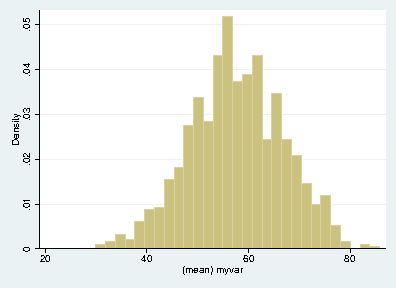
\includegraphics{images/stata_bootstrap.png}
\item
  Try it yourself!

  Download the \href{examples_Stata/bootstrap.zip}{bootstrap example files}, to
  the RCE, extract the zip file, and run the example by calling
  \texttt{condor\_submit\ bootstrap.submit} from the \texttt{bootstrap} directory.
\end{enumerate}

\hypertarget{installing-custom-software}{%
\chapter{Installing Custom Software}\label{installing-custom-software}}

\hypertarget{conda-environments}{%
\section{Conda environments}\label{conda-environments}}

The RCE is a shared resource that is actively administered to keep the cluster stable for all users. System administrators install and update software system-wide, while avoiding conflicts between software dependencies. It is not possible for RCE users to install software system-wide. However, users can install custom software into their own \emph{project shared space} if the required dependencies are already installed system-wide, or if the dependencies can also be installed into the same project space. Frequently, however, it is not possible to manually install the full suite of required software dependencies (the `dependency tree') for a given program.

A solution to this problem is to use \href{https://docs.conda.io/projects/conda/en/latest/user-guide/concepts/environments.html}{Conda environments}, which are siloed containers that can be used to install software - and their dependencies - without affecting other users on the cluster. Since Conda is a \href{https://en.wikipedia.org/wiki/Package_manager}{package management system}, it automatically handles the issue of installing appropriately versioned dependencies for any software you install.

A useful resource for interacting with Conda environments will be this \href{https://docs.conda.io/projects/conda/en/4.6.0/_downloads/52a95608c49671267e40c689e0bc00ca/conda-cheatsheet.pdf}{cheatsheet}.

\hypertarget{conda-setup}{%
\section{Conda setup}\label{conda-setup}}

Here, we walk through the steps needed to create a Conda enviroment in your \emph{project space} on the RCE.

\begin{enumerate}
\def\labelenumi{\arabic{enumi}.}
\tightlist
\item
  Start an RCE powered Anaconda shell.
\item
  Check which shell is being used and change shell to \texttt{bash} if necessary.
\end{enumerate}

\begin{Shaded}
\begin{Highlighting}[]
\OperatorTok{$}\StringTok{ }\NormalTok{echo }\OperatorTok{$}\DecValTok{0}
\OperatorTok{$}\StringTok{ }\ErrorTok{/}\NormalTok{bin}\OperatorTok{/}\NormalTok{bash }\CommentTok{\# change to bash}
\end{Highlighting}
\end{Shaded}

\begin{enumerate}
\def\labelenumi{\arabic{enumi}.}
\setcounter{enumi}{2}
\tightlist
\item
  Create a new empty Conda environment in the home directory. The \texttt{-n} option indicates the environment name comes next. After the environment name, package names (possibly multiple, separated by a space) to be installed can be listed.
\end{enumerate}

\begin{Shaded}
\begin{Highlighting}[]
\OperatorTok{$}\StringTok{ }\NormalTok{conda create }\OperatorTok{{-}}\NormalTok{n }\OperatorTok{\textless{}}\NormalTok{name}\OperatorTok{{-}}\NormalTok{of}\OperatorTok{{-}}\NormalTok{environment}\OperatorTok{\textgreater{}}
\end{Highlighting}
\end{Shaded}

\begin{enumerate}
\def\labelenumi{\arabic{enumi}.}
\setcounter{enumi}{3}
\tightlist
\item
  Make sure there is enough room in the project space to store the \texttt{.conda} folder.
\end{enumerate}

\begin{Shaded}
\begin{Highlighting}[]
\OperatorTok{$}\StringTok{ }\NormalTok{quotareport }\OperatorTok{\textasciitilde{}}\ErrorTok{/}\NormalTok{shared\_space}\OperatorTok{/}\ErrorTok{\textless{}}\NormalTok{user}\OperatorTok{{-}}\NormalTok{name}\OperatorTok{\textgreater{}}
\end{Highlighting}
\end{Shaded}

\begin{enumerate}
\def\labelenumi{\arabic{enumi}.}
\setcounter{enumi}{4}
\tightlist
\item
  Once the Conda environment is configured, use \texttt{rsync} to move (NOTE: do not use \texttt{mv} or \texttt{cp}) the \texttt{.conda} hidden directory from the home directory to a new directory (e.g., called \texttt{conda}) in the project space. Then delete the old \texttt{.conda} hidden directory within the home directory.
\end{enumerate}

\begin{Shaded}
\begin{Highlighting}[]
\OperatorTok{$}\StringTok{ }\NormalTok{rsync }\OperatorTok{{-}}\NormalTok{rav }\OperatorTok{\textasciitilde{}}\ErrorTok{/}\NormalTok{.conda }\OperatorTok{\textasciitilde{}}\ErrorTok{/}\NormalTok{shared\_space}\OperatorTok{/}\ErrorTok{\textless{}}\NormalTok{user}\OperatorTok{{-}}\NormalTok{name}\OperatorTok{\textgreater{}}\ErrorTok{/}\NormalTok{conda}
\OperatorTok{$}\StringTok{ }\NormalTok{rm }\OperatorTok{{-}}\NormalTok{r }\OperatorTok{\textasciitilde{}}\ErrorTok{/}\NormalTok{.conda}
\end{Highlighting}
\end{Shaded}

\begin{enumerate}
\def\labelenumi{\arabic{enumi}.}
\setcounter{enumi}{5}
\tightlist
\item
  Create a symbolic link (symlink) to the new directory from the original location (in the home directory). The \texttt{-s} option specifies a symlink, then the new directory is specified, then the previous location of the \texttt{.conda} folder in the home directory.
\end{enumerate}

\begin{Shaded}
\begin{Highlighting}[]
\OperatorTok{$}\StringTok{ }\NormalTok{ln }\OperatorTok{{-}}\NormalTok{s }\OperatorTok{\textasciitilde{}}\ErrorTok{/}\NormalTok{shared\_space}\OperatorTok{/}\ErrorTok{\textless{}}\NormalTok{user}\OperatorTok{{-}}\NormalTok{name}\OperatorTok{\textgreater{}}\ErrorTok{/}\NormalTok{conda}\OperatorTok{/}\NormalTok{.conda }\OperatorTok{\textasciitilde{}}\ErrorTok{/}\NormalTok{.conda}
\end{Highlighting}
\end{Shaded}

\begin{enumerate}
\def\labelenumi{\arabic{enumi}.}
\setcounter{enumi}{6}
\tightlist
\item
  View list of available Conda environments to check the symlink worked.
\end{enumerate}

\begin{Shaded}
\begin{Highlighting}[]
\OperatorTok{$}\StringTok{ }\NormalTok{conda env list}
\end{Highlighting}
\end{Shaded}

\begin{enumerate}
\def\labelenumi{\arabic{enumi}.}
\setcounter{enumi}{7}
\tightlist
\item
  Search for program(s) to install (optional). (NOTE: surround the search string with asterisks).
\end{enumerate}

\begin{Shaded}
\begin{Highlighting}[]
\OperatorTok{$}\StringTok{ }\NormalTok{conda search “}\OperatorTok{*}\NormalTok{rstan}\OperatorTok{*}\NormalTok{”}
\OperatorTok{$}\StringTok{ }\NormalTok{conda search “}\OperatorTok{*}\NormalTok{rstudio}\OperatorTok{*}\NormalTok{”}
\end{Highlighting}
\end{Shaded}

\begin{enumerate}
\def\labelenumi{\arabic{enumi}.}
\setcounter{enumi}{8}
\tightlist
\item
  Initiate the environment.
\end{enumerate}

\begin{Shaded}
\begin{Highlighting}[]
\OperatorTok{$}\StringTok{ }\NormalTok{conda activate }\OperatorTok{\textless{}}\NormalTok{name}\OperatorTok{{-}}\NormalTok{of}\OperatorTok{{-}}\NormalTok{environment}\OperatorTok{\textgreater{}}
\end{Highlighting}
\end{Shaded}

\begin{enumerate}
\def\labelenumi{\arabic{enumi}.}
\setcounter{enumi}{9}
\tightlist
\item
  Install new programs into this active environment.
\end{enumerate}

\begin{Shaded}
\begin{Highlighting}[]
\OperatorTok{$}\StringTok{ }\NormalTok{conda install r}\OperatorTok{{-}}\NormalTok{rstan rstudio}
\end{Highlighting}
\end{Shaded}

For some programs / packages, you may need to specify a non-default Conda channel using the flag \texttt{-c\ \textless{}channel-name\textgreater{}}. See \url{https://docs.conda.io/projects/conda/en/latest/user-guide/concepts/channels.html} for more information.

\begin{Shaded}
\begin{Highlighting}[]
\OperatorTok{$}\StringTok{ }\NormalTok{conda install }\OperatorTok{{-}}\NormalTok{c conda}\OperatorTok{{-}}\NormalTok{forge r}\OperatorTok{{-}}\NormalTok{nbclust}
\end{Highlighting}
\end{Shaded}

\begin{enumerate}
\def\labelenumi{\arabic{enumi}.}
\setcounter{enumi}{10}
\tightlist
\item
  Check where program(s) are installed and which version (optional).
\end{enumerate}

\begin{Shaded}
\begin{Highlighting}[]
\OperatorTok{$}\StringTok{ }\NormalTok{which R}
\OperatorTok{$}\StringTok{ }\NormalTok{which python}
\OperatorTok{$}\StringTok{ }\NormalTok{R }\OperatorTok{{-}{-}}\NormalTok{version}
\OperatorTok{$}\StringTok{ }\NormalTok{echo }\OperatorTok{$}\NormalTok{PATH}
\end{Highlighting}
\end{Shaded}

\begin{enumerate}
\def\labelenumi{\arabic{enumi}.}
\setcounter{enumi}{11}
\tightlist
\item
  Run a program.
\end{enumerate}

\begin{Shaded}
\begin{Highlighting}[]
\OperatorTok{$}\StringTok{ }\NormalTok{R}
\OperatorTok{$}\StringTok{ }\NormalTok{rstudio}
\end{Highlighting}
\end{Shaded}

\begin{enumerate}
\def\labelenumi{\arabic{enumi}.}
\setcounter{enumi}{12}
\tightlist
\item
  Deactivate environment after use.
\end{enumerate}

\begin{Shaded}
\begin{Highlighting}[]
\OperatorTok{$}\StringTok{ }\NormalTok{conda deactivate}
\end{Highlighting}
\end{Shaded}

\textbf{NOTE:} if you need to move your existing Conda environment directory to a different location, it's best to remove the old \texttt{.conda} directory and start with a fresh one in the new location.

\end{document}
